\documentclass[11pt, a4paper]{article}
\usepackage{graphicx}
\usepackage{amsmath}
\usepackage{listings}
\usepackage{minted}
\usepackage{physics}

\title{ASSIGNMENT 7: CIRCUIT ANALYSIS USING SYMPY AND LAPLACE TRANSFORMS}
\author{Nithin Babu [EE18B021]}
\date{\today}

\begin{document}
\maketitle

\section*{Abstract}
The goal of this assignment is the following:
\begin{itemize}
\item To analyze Filters using Laplace Transform.
\item To see how python can be used for symbolic Algebra.
\item To plot graphs to understand high pass and low pass analog filters.
\end{itemize}

\section*{Low Pass Filter}
The low pass filter that we use gives the following matrix equation after simplification of the modified nodal equations.
\[\begin{pmatrix} 0 & 0 & 1 & -\frac{1}{G} \\ -\frac{1}{1+sR_2C_2} & 1 & 0 & 0 \\ 0 & -G & G & 1 \\ -\frac{1}{R_1}-\frac{1}{R_2}-sC_1 & \frac{1}{R_2} & 0 & sC_1 \end{pmatrix}\begin{pmatrix} V_1 \\ V_p \\ V_m \\ V_o \end{pmatrix} = \begin{pmatrix} 0 \\ 0 \\ 0 \\ -V_i(s)/R_1 \end{pmatrix}\]

The python code snippet that declares the low pass function and solves the matrix equation to get the V matrix is as shown below:
\begin{minted}{python3}
# Declaring the sympy function for a lowpass filter.
def lowpass(R1,R2,C1,C2,G,Vi):
	s = symbols('s')
# Creating the matrices and solving them to get the output voltage.	
	A = Matrix([[0,0,1,-1/G],
		[-1/(1+s*R2*C2),1,0,0],
		[0,-G,G,1],
		[-1/R1-1/R2-s*C1,1/R2,0,s*C1]])
	b = Matrix([0,0,0,-Vi/R1])
	V = A.inv()*b
	return A,b,V
\end{minted}
The plot for the magnitude of the transfer function (magnitude bode plot) is as shown below:
\begin{figure}[!tbh]
   	\centering
   	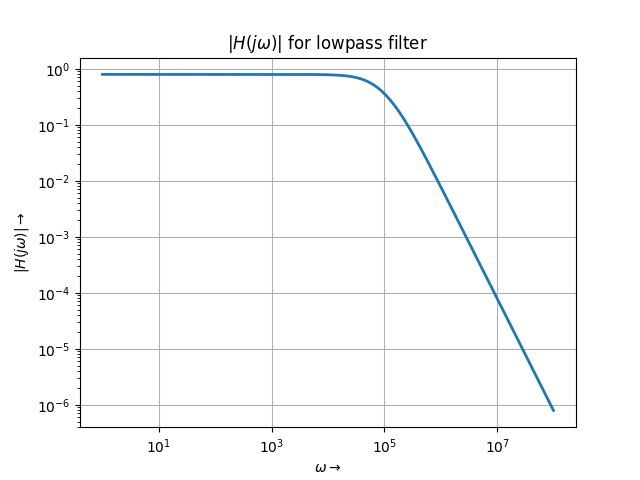
\includegraphics[scale=0.6]{Figure_0.png}
   	\label{fig:32}
   	\caption{Magnitude bode plot of the low pass filter}
   \end{figure}

\section*{High Pass Filter}
The high pass filter we use gives the following matrix equations after simplification of the modified nodal equations
\[\begin{pmatrix} 0 & 0 & 1 & -\frac{1}{G} \\ -\frac{-sR_3C_2}{1+sR_3C_2} & 1 & 0 & 0 \\ 0 & -G & G & 1 \\ -1-(sR_1C_1)-(sR_3C_2)) & sC_2R_1 & 0 & 1 \end{pmatrix}\begin{pmatrix} V_1 \\ V_p \\ V_m \\ V_o \end{pmatrix} = \begin{pmatrix} 0 \\ 0 \\ 0 \\ -V_i(s)sR_1C_1 \end{pmatrix}\]

The python code snippet that declares the high pass function and solves the matrix equation to get the V matrix is as shown below:

\begin{minted}{python3}
# Declaring the sympy function for a highpass filter.
def highpass(R1,R3,C1,C2,G,Vi):
    s = symbols("s")
# Creating the matrices and solving them to get the output voltage.	
    A = Matrix([[0,-1,0,1/G],
        [s*C2*R3/(s*C2*R3+1),0,-1,0],
        [0,G,-G,1],
        [-s*C2-1/R1-s*C1,0,s*C2,1/R1]])
    b = Matrix([0,0,0,-Vi*s*C1])
    V = A.inv()*b
    return A,b,V
\end{minted}
The plot for the magnitude of the transfer function (magnitude bode plot) is as shown below:
\begin{figure}[!tbh]
   	\centering
   	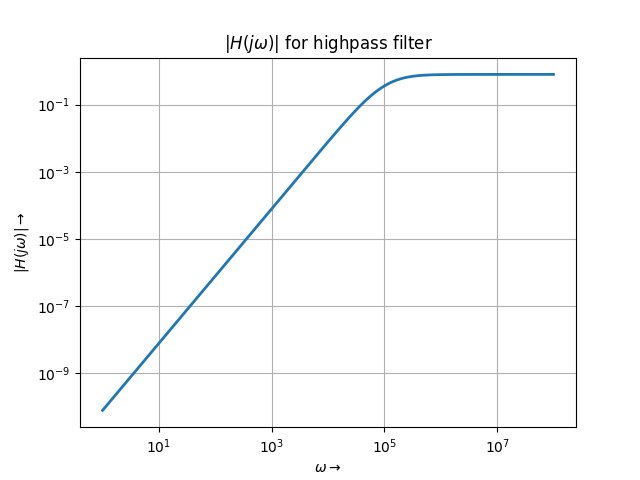
\includegraphics[scale=0.6]{Figure_3.png}
   	\label{fig:32}
   	\caption{Magnitude bode plot of the high pass filter}
   \end{figure}
\section*{Format Change of Sympy Functions}
The sympy functions,that are expressed in terms of 's', must be converted to another form that is understood by sp.signal. This is done using the \textit{sympyToTrFn()} function.\\
The python code snippet is as shown:
\begin{minted}{python3}
# Creating a function to convert a sympy function into a version 
# that is understood by sp.signal  	 
def sympyToTrFn(Y):
# The below line will simplify the expression and give it in Nr/Dr form.	
    Y = expand(simplify(Y))
# The following lines will give the proper form for numerator and denomerator.    
    n,d = fraction(Y)
    n,d = Poly(n,s), Poly(d,s)
    num,den = n.all_coeffs(), d.all_coeffs()
    num,den = [float(f) for f in num], [float(f) for f in den]
# This will calculate the function that is understood by sp.signal    
    H = sp.lti(num,den)
    return H
\end{minted}

\section*{Step Response Of the Low Pass Filter}
In order to find the step response of the low pass filter, we need to assign $ Vi(s) = 1/s $. 
The python code below explains it. 
\begin{minted}{python3}
# These lines of code will calculate the step response for the lowpass filter.
A1,b1,V1 = lowpass(10000,10000,1e-9,1e-9,1.586,1/s)
Vo1 = V1[3]
H1 = sympyToTrFn(Vo1)
t,y1 = sp.impulse(H1,None,p.linspace(0,5e-3,10000))

# The plot for step response of a lowpass filter.
p.figure(1)
p.plot(t,y1)
p.title(r"Step Response for low pass filter")
p.xlabel(r'$t\rightarrow$')
p.ylabel(r'$V_o(t)\rightarrow$')
p.grid(True)
p.show()
\end{minted}
The plot for the step response of the low pass circuit is as shown:
\begin{figure}[!tbh]
   	\centering
   	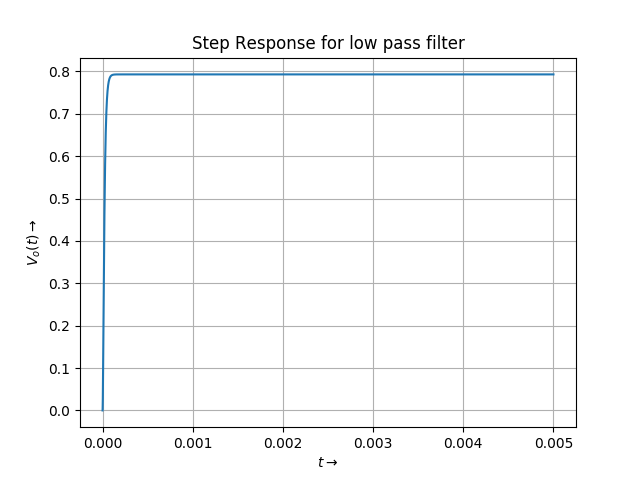
\includegraphics[scale=0.6]{Figure_1.png}
   	\label{fig:32}
   	\caption{Step response of low pass filter.}
   \end{figure}
\section*{Response to Sum Of Sinusoids}   
    When the input is a sum of sinusoids like,
\begin{equation*}
  V_{i}(t) = ( \ \sin(2000\pi t) + \cos(2*10^{6}\pi t) \ )u_{o}(t) \ Volts
  \end{equation*}
  Then the output response for the lowpass filter can easily be found as shown in the code snippet.
  \begin{minted}{python3}
# The below piece of code will calculate the transfer function for the lowpass filter.
s = symbols('s')
A,b,V = lowpass(10000,10000,1e-9,1e-9,1.586,1)
Vo = V[3]
H = sympyToTrFn(Vo)
ww = p.logspace(0,8,801)
ss = 1j*ww
hf = lambdify(s,Vo,'numpy')
v = hf(ss)

# The response is also calculated for sum of sinusoids.
vi = p.sin(2000*pi*t) + p.cos(2e6*pi*t)
t,y2,svec = sp.lsim(H,vi,t)
# The plot for output response for sum of sinusoids of a lowpass filter.
p.figure(2)
p.plot(t,y2)
p.title(r"Output voltage for sum of sinusoids")
p.xlabel(r'$t\rightarrow$')
p.ylabel(r'$V_o(t)\rightarrow$')
p.grid(True)
p.show()
  \end{minted}
The output response to the sum of sinusoids for the low pass filter is as shown:
\begin{figure}[!tbh]
   	\centering
   	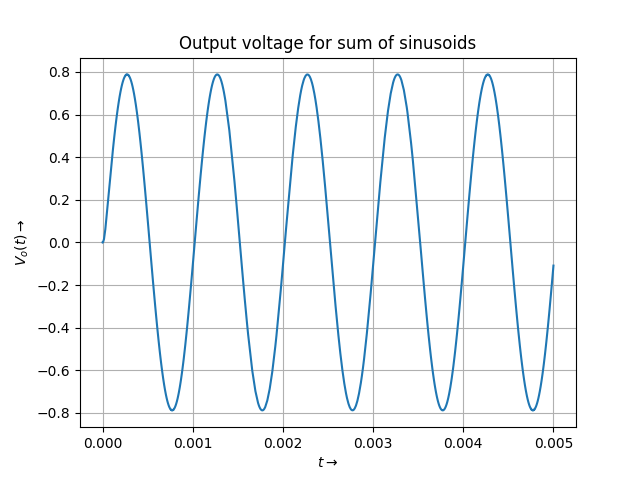
\includegraphics[scale=0.6]{Figure_2.png}
   	\label{fig:32}
   	\caption{Output response to the sum of sinusoids.}
   \end{figure}
   \newpage
\section*{Response to Damped Sinusoids}
In this case we assign the input voltage as a damped sinusoid like,\\
Low frequency,
\begin{equation*}
    V_{i}(t) = e^{-500t}( \ \cos(2000\pi t) \ )u_{o}(t) \ Volts
\end{equation*}
High frequency,
\begin{equation*}
    V_{i}(t) = e^{-500t}( \ \cos(2*10^{6}\pi t) \ )u_{o}(t) \ Volts
\end{equation*}
The high frequency and low frequency plots of the input damped sinusoids are as shown:\newpage
\begin{figure}[!tbh]
   	\centering
   	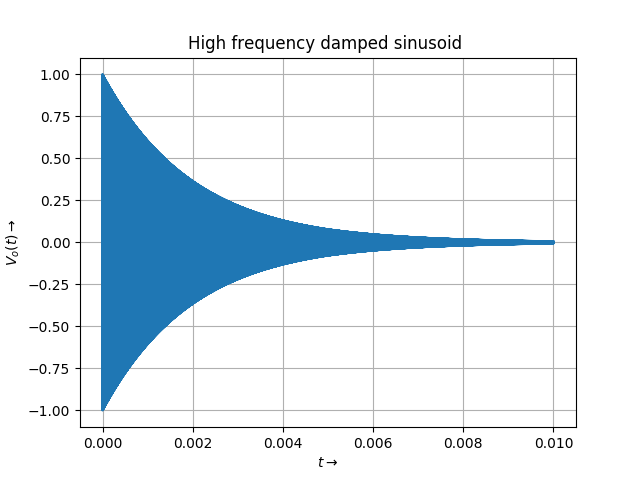
\includegraphics[scale=0.6]{Figure_4.png}
   	\label{fig:32}
   	\caption{High frequency damped sinusoid}
   \end{figure}
\begin{figure}[!tbh]
   	\centering
   	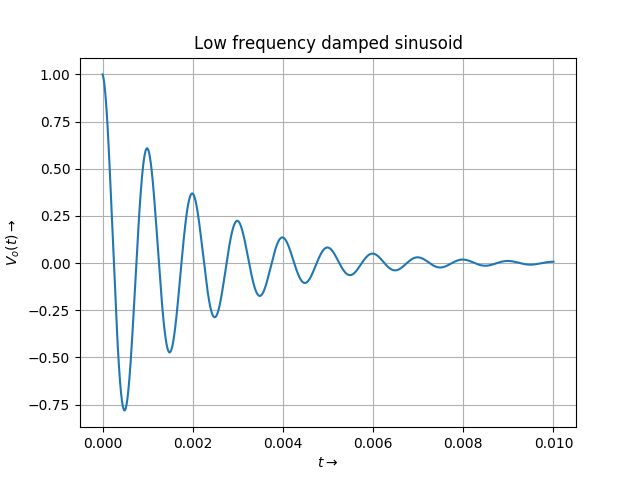
\includegraphics[scale=0.6]{Figure_5.png}
   	\label{fig:32}
   	\caption{Low frequency damped sinusoid}
   \end{figure}
The python code snippet to execute the above is as shown:
\begin{minted}{python3}
# The below piece of code will calculate the transfer function
# for the highpass filter.
A3,b3,V3 = highpass(10000,10000,1e-9,1e-9,1.586,1)
Vo3 = V3[3]
H3 = sympyToTrFn(Vo)
hf3 = lambdify(s,Vo3,'numpy')
v3 = hf3(ss)

# The output response is calculated when the input is a damped sinusoid 
#for both high and low frequency.

# High frequency.
damping_factor = -500
t2 = p.linspace(0,1e-2,1e5) 
vi4_1 = p.exp(damping_factor*t2)*p.cos(2e6*pi*t2)
t2,y4_1,svec = sp.lsim(H3,vi4_1,t2)

# Low frequency.
t3 = p.linspace(0,1e-2,1e5)
vi4_2 = p.exp(damping_factor*t3)*p.cos(2e3*pi*t3)
t3,y4_2,svec = sp.lsim(H3,vi4_2,t3)

# The plot for high frequency damped sinusoid response from highpass filter.
p.figure(6)
p.plot(t2,y4_1)
p.title(r"High frequency damped sinusoid response from High Pass filter")
p.xlabel(r'$t\rightarrow$')
p.ylabel(r'$V_o(t)\rightarrow$')
p.grid(True)

# The plot for low frequency damped sinusoid response from highpass filter.
p.figure(7)
p.plot(t3,y4_2)
p.title(r"Low frequency damped sinusoid response from High Pass filter")
p.xlabel(r'$t\rightarrow$')
p.ylabel(r'$V_o(t)\rightarrow$')
p.grid(True)
p.show()	
\end{minted}

The output responses for both cases in a high pass filter is as shown:\newpage
\begin{figure}[!tbh]
   	\centering
   	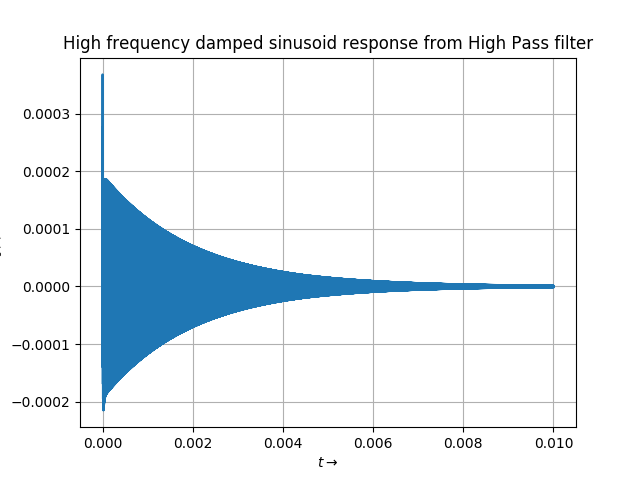
\includegraphics[scale=0.6]{Figure_6.png}
   	\label{fig:32}
   	\caption{Output response of a high frequency damped sinusoid}
   \end{figure}
\begin{figure}[!tbh]
   	\centering
   	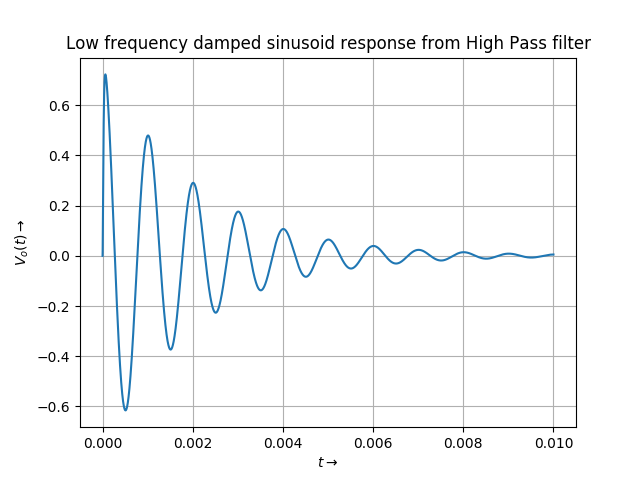
\includegraphics[scale=0.6]{Figure_7.png}
   	\label{fig:32}
   	\caption{Output response of a low frequency damped sinusoid}
   \end{figure}

\section*{Step Response of High Pass Filter}
In order to find the step response of the high pass filter, we need to assign $ Vi(s) = 1/s $. 
The python code below explains it.
\begin{minted}{python3}
# The step response is calculated for a highpass filter.
A5,b5,V5 = highpass(10000,10000,1e-9,1e-9,1.586,1/s)
Vo5 = V5[3]
H5 = sympyToTrFn(Vo5)
t5,y5 = sp.impulse(H5,None,p.linspace(0,5e-3,10000))

# The plot for step response of a highpass filter.
p.figure(8)
p.plot(t5,y5)
p.title(r"Step Response for high pass filter")
p.xlabel(r'$t\rightarrow$')
p.ylabel(r'$V_o(t)\rightarrow$')
p.grid(True)
p.show()	
\end{minted}
The plot of the step response for a high pass filter is as shown:
\begin{figure}[!tbh]
   	\centering
   	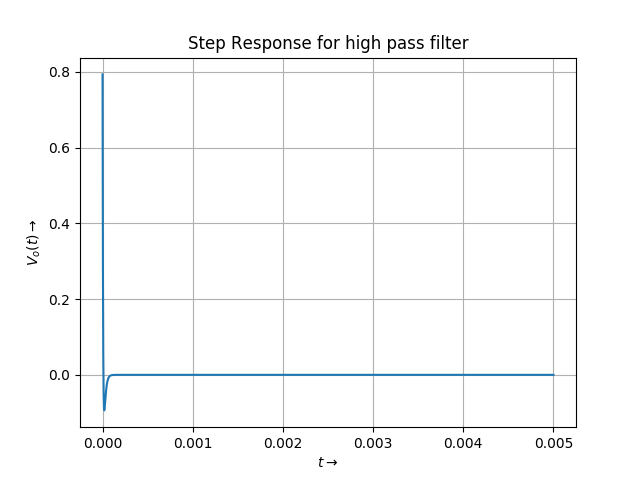
\includegraphics[scale=0.6]{Figure_8.png}
   	\label{fig:32}
   	\caption{Step response for a high pass filter}
   \end{figure}\newpage
The unit step response, as expected is high at t=0 when there is an abrupt
change in the input. Since there is no other change at large time values outside
the neighbourhood of 0, the Fourier transform of the unit step has high values
near 0 frequency, which the high pass filter attenuates.

\section*{Conclusion}
In conclusion, the sympy module has allowed us to analyse quite complicated circuits by analytically solving their node equations. We then interpreted the solutions by plotting time domain responses using the signals toolbox. Thus, sympy combined with the scipy.signal module is a very useful toolbox for analyzing complicated systems like the active filters in this assignment.   
\end{document}


